% Copyright 2021 Edoardo Riggio

% Licensed under the Apache License, Version 2.0 (the "License");
% you may not use this file except in compliance with the License.
% You may obtain a copy of the License at

% 	http://www.apache.org/licenses/LICENSE-2.0

% Unless required by applicable law or agreed to in writing, software
% distributed under the License is distributed on an "AS IS" BASIS,
% WITHOUT WARRANTIES OR CONDITIONS OF ANY KIND, either express or implied.
% See the License for the specific language governing permissions and
% limitations under the License.

\documentclass{article}

\usepackage{hyperref, amsmath, graphicx, amssymb}
\usepackage{fancyvrb, newverbs, xcolor, tikz}
\usepackage[latin1]{inputenc}

\usetikzlibrary{positioning}

\graphicspath{{./assets/}}
\definecolor{cverbbg}{gray}{0.93}

\newenvironment{cverbatim}
 {\SaveVerbatim{cverb}}
 {\endSaveVerbatim
  \flushleft\fboxrule=0pt\fboxsep=.5em
  \colorbox{cverbbg}{\BUseVerbatim{cverb}}%
  \endflushleft
}

\newenvironment{lcverbatim}
 {\SaveVerbatim{cverb}}
 {\endSaveVerbatim
  \flushleft\fboxrule=0pt\fboxsep=.5em
  \colorbox{cverbbg}{%
    \makebox[\dimexpr\linewidth-2\fboxsep][l]{\BUseVerbatim{cverb}}%
  }
  \endflushleft
}

\begin{document}
\begin{titlepage}
    \begin{center}
        \vspace*{1cm}
        
        \Huge
        \textbf{Theory of Computation Cheatsheet}
        
        \vspace{0.5cm}
        \LARGE
        
        \vspace{.5cm}
        
        Edoardo Riggio
   		  \vspace{1.5cm}
       
        \vfill
        
        \today
        
        \vspace{.8cm}
          \Large
          Theory of Computation - S.P. 2022 \\
        Computer Science\\
        Universit\`{a} della Svizzera Italiana, Lugano\\
        
    \end{center}
\end{titlepage}

\tableofcontents

\newpage

\section{Introduction}
The Turing Machine was invented by \textbf{Alan Turing} in 1936. A Turing Machine is a much more accurate model of a general-purpose computer than a PDA or FA. This type of machine can do anything that a real computer can. \\ \\
The following are some characteristics of a Turing Machine:

\begin{itemize}
	\item The input tape of the TM is infinite
	\item The input head of the TM can both read from and write to the tape
	\item The input head of the TM can move both left and right
	\item The RM has both accepting and rejecting states. Once it reaches such states, it accepts/rejects immediately -- i.e., it does not need to get to the end of the input.
\end{itemize}

\subsection{Formal Definition}
A Turing Machine is defined as follows:
\[ TM: (Q, \Sigma, G, \delta, q_0, q_{accept}, q_{reject}) \]
Where $Q$ is a \textbf{set of states}, $\Sigma$ is the \textbf{input alphabet}, $G$ is the \textbf{tape alphabet} -- where $\Sigma \subset G$, $\delta$ is the \textbf{transition function}, $q_0$ is the \textbf{initial state}, $q_{accept}$ is the \textbf{set of accepting states}, and $q_{reject}$ is the \textbf{set of rejecting states}.

\subsection{Configurations}
\subsubsection{Starting Configuration}
The starting configuration of $M$ on $\omega$ is $q_0 \omega$, which indicates that the machine is in the start stating state $q_0$. Moreover, the head of the TM is in the leftmost position.

\subsubsection{Accepting and Rejecting Configurations}
The accepting and rejecting configurations are the halting configurations. They do not yield any further configuration.

\subsection{Acceptance}
A Turing Machine is said to accept an input string $\omega$ if a sequence of configurations $C_1, C_2, \dots C_k$ exists where:

\begin{itemize}
	\item $C_1$ is the starting configuration
	\item $C_i$ yields $C_{i+1}$
	\item $C_k$ is the accepting configuration
\end{itemize}

\subsection{Turing-Recognizable Language}
A collection of strings is called the language of a TM if the TM \textbf{accepts} it. A TM is said to \textbf{recognize} a language if it accepts all and only those strings in the language. \\ \\
A language is said to be \textbf{Turing-recognizable} if some TM recognizes it. This means that a TM can accept, reject or loop.

\subsection{Turing-decidable Language}
While the possible outcomes of a TM are \textit{accept}, \textit{reject} and \textit{loop}, a TM \textbf{decides} a language if it accepts all strings in the language, and reject all strings not in the language -- i.e., it never loops.

\subsection{Turing Machine Variants}
\subsubsection{Multitape Turing Machines}
This is a TM that has $k$ number of tapes. The transition function for this Turing Machine allows for reading, writing, and moving the heads on some or all tapes simultaneously. \\ \\
Every multitape Turing Machine has an equivalent single-tape Turing Machine.

\subsubsection{Non-Deterministic Turing Machines}
The machine may proceed according to several different choices at any point in the computation. The resulting computation is a tree whose branches correspond to the various possibilities of the machine. \\ \\
A non-deterministic Turing Machine \textbf{accepts} if some branch of the computation leads to an accepting state. \\ \\
Every nondeterministic Turing Machine has an equivalent deterministic Turing Machine.

\section{Computability Theory}
We study unsolvability because knowing a problem cannot be solved helps us restate or simplify the problem.

\subsection{Solvability}
A problem is said to be solvable if we can find a Turing Machine that \textbf{decides} that problem.

\begin{center}
	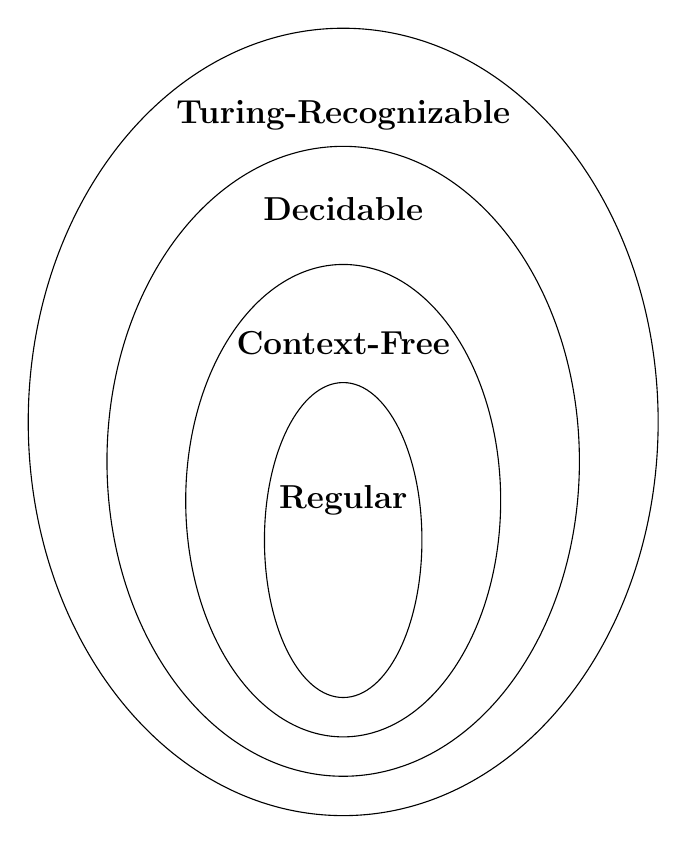
\begin{tikzpicture}
    	\begin{scope}
          \draw[draw = black] (0,0) ellipse (4 and 5);
      	  \draw[draw = black] (0,-0.5) ellipse (3 and 4);
       	  \draw[draw = black] (0,-1) ellipse (2 and 3);
      	  \draw[draw = black] (0,-1.5) ellipse (1 and 2);
    		\node at (0,3.9) (A) {\large\textbf{Turing-Recognizable}};
    		\node at (0,2.7) (B) {\large\textbf{Decidable}};
    		\node at (0,1) (C) {\large\textbf{Context-Free}};
    		\node at (0,-1) (C) {\large\textbf{Regular}};
    	\end{scope}

	\end{tikzpicture}
\end{center}

\subsection{Decidabile Problems}
Showing that a language is decidable is the same as showing that the computational problem is decidable.

\subsubsection{DFA Acceptance Problem}
The language $A_{DFA}$ is decidable. To prove it, we need to build a Turing Machine $M$ that decides $A_{DFA}$. \\ \\
$M$ = On input $\langle B, \omega\rangle$, where $B$ is a DFA and $\omega$ is a string:

\begin{enumerate}
	\item Simulate $B$ on $\omega$
	\item If the simulation ends in an accepting state \textbf{accept}, otherwise \textbf{reject}
\end{enumerate}

\subsubsection{NFA Acceptance Problem}
The language $A_{NFA}$ is decidable. To prove it, we need first to convert the NFA into a DFA and then apply the same procedure as the one in the $A_{DFA}$ proof. \\ \\
$N$ = On input $\langle B, \omega \rangle$, where $B$ is an NFA and $\omega$ is a string:

\begin{enumerate}
	\item Convert $B$ into an equivalent DFA $C$
	\item Simulate $C$ on $\omega$
	\item If the simulation ends in an accepting state \textbf{accept}, otherwise \textbf{reject}
\end{enumerate}

\subsubsection{DFA Emptiness Problem}
The language $E_{DFA}$ is decidable. We need to check if we can reach an accepting state by traveling the DFA to prove it. \\ \\
$S$ = On input $\langle A \rangle$, where $A$ is a DFA:

\begin{enumerate}
	\item Mark the starting state of the DFA
	\item Continue marking the states of the DFA until no new state gets marked
	\item If, once all states have been marked, no accept state was marked, \textbf{accept}, otherwise \textbf{reject}
\end{enumerate}

\subsubsection{DFA Equivalence Problem}
The language $EQ_DFA$ is decidable. We need to build an automaton that checks if both DFAs or neither accepts the string to prove it. \\ \\
$M$ = On input $\langle A, B \rangle$ where both $A$ and $B$ are DFAs:

\begin{enumerate}
	\item Construct a DFA $C$ with symmetric difference feature. If two automata recognize the same language, the newly constructed automaton accepts nothing when the languages are the same.
	\item Feed the newly constructed DFA to $M$
	\item Mark the starting state of $C$
	\item Continue marking the states of the DFA until no new state gets marked
	\item If, once all states have been marked, no accept state was marked, \textbf{accept}, otherwise \textbf{reject}
\end{enumerate}

\subsubsection{CFG Emptiness Problem}
The language $E_{CFG}$ is decidable. To prove it, we construct a Turing machine $M$. \\ \\
$M$ = On input $\langle G \rangle$, where $G$ is a CFG:

\begin{enumerate}
	\item Mark all terminal symbols in $G$
	\item Repeat this operation until no new varibale gets marked
	\item If, once all varibles have been marked, the start variable was not marked \textbf{accept}, otherwise \textbf{reject}
\end{enumerate}

\end{document}

































